\documentclass[letterpaper]{article}
\usepackage{aaai}
\usepackage{times}
\usepackage{helvet}
\usepackage{courier}
\usepackage{amsmath,amsfonts,amssymb,amsthm}
\usepackage{array}
\usepackage{amsmath,amssymb}
\usepackage{epsfig,subfigure}
\usepackage[vlined,algoruled,titlenumbered,noend]{algorithm2e}
\frenchspacing

\newtheorem{lemma}{Lemma}
\newtheorem{assumption}[lemma]{Assumption}
\newtheorem{restr}{Restriction}   %[section]
\newtheorem{theorem}[lemma]{Theorem}
\newtheorem{proposition}[lemma]{Proposition}
\newtheorem{corollary}[lemma]{Corollary}
\newtheorem{hypothesis}[lemma]{Hypothesis}
\newtheorem{definition}[lemma]{Definition}

\usepackage[vlined,algoruled,titlenumbered,noend]{algorithm2e}
%\usepackage{proceed2e}

% If your paper is accepted and the title of your paper is very long,
% the style will print as headings an error message. Use the following
% command to supply a shorter title of your paper so that it can be
% used as headings.
%
%\runningtitle{I use this title instead because the last one was very long}

% If your paper is accepted and the number of authors is large, the
% style will print as headings an error message. Use the following
% command to supply a shorter version of the authors names so that
% they can be used as headings (for example, use only the surnames)
%
%\runningauthor{Surname 1, Surname 2, Surname 3, ...., Surname n}

\newcommand{\fix}{\marginpar{FIX}}
\newcommand{\new}{\marginpar{NEW}}
\newcommand{\ind}[1]{\mathbb{I}[#1]}
\newcommand{\inde}{\mathbb{I}}

\newcommand{\var}{v}
\newcommand{\eq}{\leftarrow}

\newcommand{\LB}{\mathit{LB}}
\newcommand{\UB}{\mathit{UB}}

\newcommand{\B}{\mathbb{B}}
\newcommand{\E}{\mathbb{E}}
\newcommand{\I}{\mathbb{I}}
\newcommand{\R}{\mathbb{R}}
\renewcommand{\vec}[1]{\mathbf{#1}}

%%%%%%%%%%
% PDFINFO for PDFTEX
% Uncomment and complete the following for metadata if
% your paper is typeset using PDFTEX
% npdfinfof
\pdfinfo{
/Title (Symbolic Variable Elimination for Discrete and Continuous Graphical Models)
/Author (Scott Sanner and Ehsan Abbasnejad)
/Subject (Proceedings of the Twenty-sixth AAAI Conference (AAAI-12))
/Keywords (Graphical Models, Dynamic Programming, Hybrid Discrete and ContinuousProbabilistic Inference)
}
%%%%%%%%%%

\setcounter{secnumdepth}{0}  

\begin{document}

\title{Symbolic Variable Elimination for Discrete and Continuous Graphical Models}
\author{Scott Sanner\\
NICTA \& ANU\\
Canberra, Australia\\
{\tt ssanner@nicta.com.au}
\And
Ehsan Abbasnejad\\
ANU \& NICTA\\
Canberra, Australia\\
{\tt ehsan.abbasnejad@anu.edu.au}
}

% TODO:
% - replace inference examples
% - emphasize oblique
% - add references to MTEs in Related Work... save .bbl
% - arbitrary expectations of polynomials?
% - computational complexity

\maketitle
\begin{abstract}
\begin{quote}
Probabilistic reasoning in the real-world often requires inference in
continuous variable graphical models, yet there are few methods for
\emph{exact, closed-form} inference when joint distributions are
non-Gaussian.  To address this inferential deficit, we introduce SVE
-- a \emph{symbolic} extension of the well-known \emph{variable
elimination} algorithm to perform exact inference in an
\emph{expressive} class of mixed discrete and continuous variable
graphical models whose conditional probability functions can be
well-approximated as oblique piecewise polynomials with
bounded support.  Using this representation, we show that we can
compute all of the SVE operations \emph{exactly and in closed-form},
which crucially includes \emph{definite integration w.r.t.\ multivariate 
piecewise polynomial functions}.  To aid in the efficient computation
and compact representation of this solution, we use an extended
algebraic decision diagram (XADD) data structure that supports all SVE
operations.  We provide illustrative results for SVE on probabilistic
inference queries inspired by robotics localization and tracking
applications that mix various continuous distributions; this
represents the first time a general closed-form exact solution
has been proposed for this expressive class of discrete/continuous
graphical models.
\end{quote}
\end{abstract}

\section{Introduction}

\label{sec:intro}

% Max function
% Dynamics
% Expectations of arbitrary functions if allowing delta function!

% Conditions for delta: 
% - either a Bayesian network (so parents form DAG), or a 
% - factor graph where delta connects disconnected components
%   for LHS and RHS (removal of delta leads to disconnection)
%delta(x=y)
%delta(y=z)
%delta(z=x)

% Probabilities
% Expectations
% Expected risk <- risk example of why multimodal distributions
%                  should not be approximated by unimodal distributions
% (A paper on ``symbolic Bayesian decision theory''... both
%  the risk integrals and expressive functions / delta functions
%  as well as maybe the uniform polyhedra approach.)
% (Decision theory adds piecewise boundaries!)

Real-world probabilistic reasoning is rife with 
uncertainty over continuous random variables with
complex (often nonlinear) relationships, e.g.,
estimating the position and pose of entities from 
measurements in robotics, or radar tracking
applications with asymmetric stochastic dynamics and complex mixtures of 
noise processes.
While closed-form exact solutions exist for inference in some
continuous variable graphical models, such solutions are largely
limited to relatively well-behaved cases such as joint Gaussian
models.  On the other hand, the more complex inference tasks of
tracking with real-world sensors involves underlying distributions
that are beyond the reach of current closed-form exact solutions.
Take, for example, the robot sensor model in Figure~\ref{fig:gm2} 
motivated by~\cite{thrun_mcl}.
%%%%%%%%%%%%%%%%%%%%%%%%%%%%%%%%%%%%%%%%%%%%%%%%%%%%%%%%%%%%%%%%%%%%%%%%%%
%\begin{minipage}{\textwidth}
\begin{figure}%[th!]
\begin{center}
\vspace{-1mm}
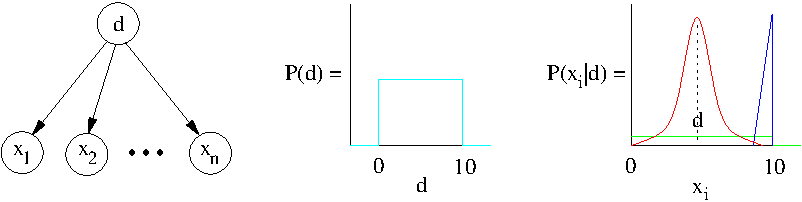
\includegraphics[width=.48\textwidth]{Figs/gm2.pdf}
\end{center}
\vspace{-6mm}
\caption{\footnotesize The \emph{robot localization} graphical model and all conditional probabilities.} \label{fig:gm2}
%\caption{\footnotesize .} 
\vspace{-4mm}
\end{figure}
%\end{minipage}
%%%%%%%%%%%%%%%%%%%%%%%%%%%%%%%%%%%%%%%%%%%%%%%%%%%%%%%%%%%%%%%%%%%%%%%%%%
Here $d \in \R$ is a variable representing the distance of a
mobile robot to a wall and $x_i$ are the observed measurements of
distance (e.g., using a laser range finder).  The prior distribution
$P(d)$ is uniform $U(d;0,10)$ while the observation model
$P(x_i|d)$ is a \emph{mixture} of three distributions: (red) is a
truncated Gaussian 
representing noisy measurements $x_i$ of the actual
distance $d$ within the sensor range of $[0,10]$; 
(green) is a uniform noise model $U(d;0,10)$
representing random anomalies leading to any measurement; and
(blue) is a triangular distribution peaking at the maximum measurement
distance (e.g., caused by spurious deflections of laser light or the 
transparency of glass).

While our focus in this paper is on exact inference in \emph{general}
discrete and continuous variable graphical models and not purely on
this robotics localization task, this example clearly motivates the
real-world need for reasoning with complex distributions over
continuous variables.  However, in contrast to previous work that has
typically resorted to (sequential) Monte Carlo
methods~\cite{thrun_mcl,particle_filters} to perform inference in this
model (and dynamic extensions) via 
\emph{sampling}, our point of departure in this work is to seek \emph{exact,
closed-form solutions} to general probabilistic inference tasks in
these graphical models, e.g., arbitrary conditional probability 
queries or conditional expectation computations.

To achieve this task, we focus on an expressive class of mixed
discrete and continuous variable Bayesian networks whose conditional
probability functions can be expressed as oblique piecewise polynomials with
bounded support (where oblique piece boundaries are represented
by conjunctions of linear inequalities).  
In practice, this representation is sufficient to
represent or arbitrarily approximate a wide range of common
distributions such as the following: uniform (piecewise constant),
triangular (piecewise linear), truncated normal
distributions\footnote{In practice, measurements have natural ranges
that make truncated variants of distributions appropriate, e.g., a
range finder that exhibits Gaussian distributed measurement errors but
only returns measurements in the range $[0,10]$ may be well-suited to
a truncated Normal distribution observation model.}  (piecewise
quadratic or quartic), as well as all mixtures of such distributions
as exemplified in $P(x_i|d)$ above (since a sum of piecewise
polynomials is still piecewise polynomial).  While polynomials
directly support the integrals we will need to compute \emph{variable
elimination}~\cite{varelim} in closed-form, computing the definite
integrals of polynomials w.r.t.\ arbitrary linear piece boundaries
turns out to be a much more difficult task achieved through novel
\emph{symbolic} methods that underlie the key contribution of
\emph{symbolic variable elimination (SVE)} that we make in this paper.

% E[d|x_1] example?
In the following sections, we present our graphical model
framework using a \emph{case} representation of probability
distributions followed by a description of our SVE procedure.  
After this, we introduce
the \emph{extended algebraic decision diagram (XADD)} --- a practical
data structure for efficiently and compactly manipulating the case
representation --- and apply XADD-based SVE to robotics localization 
and a tracking tasks demonstrating exact closed-form inference 
for these problems.  

\section{Discrete and Continuous Graphical Models}

\subsection{Factor Graph Representation}

A discrete and continuous \emph{graphical model} compactly represents
a joint probability distribution $p(\vec{b},\vec{x})$ over an
assignment $(\vec{b},\vec{x}) = ( b_1,\ldots,b_n,x_{1},\ldots,x_m )$
to respective random variables $(\vec{B},\vec{X}) =
(B_1,\ldots,B_n,X_{1},\ldots,X_m )$.\footnote{Notational comments:
we sometimes abuse notation and treat
vectors of random variables or assignments as a set, e.g., 
$(\vec{b},\vec{x}) = \{ b_1,\ldots,b_n,x_1,\ldots,x_m \}$.  
Also we often do
not distinguish between a random variable (upper case) and its
realization (lower case), e.g., $p(x_1) := p(X_1 = x_1)$.}  Each $b_i$
($1 \leq i \leq n$) is boolean s.t.\ $b_i \in \{ 0,1 \}$ and each
$x_j$ ($1 \leq j \leq m$) is continuous s.t.\ $x_j \in \R$.

As a general representation of both directed and undirected graphical
models, we use a \emph{factor graph}~\cite{factor_graph} 
representing a joint probability $p(\vec{b},\vec{x})$ as a
product of a finite set of factors $F$, i.e.,
\vspace{-2mm}
{\footnotesize
\begin{equation}
p(\vec{b},\vec{x}) = \frac{1}{Z} \prod_{f \in F} \Psi_f(\vec{b}_f,\vec{x}_f).
\label{eq:fg}
\vspace{-1mm}
\end{equation}
}
Here, $\vec{b}_f$ and $\vec{x}_f$ denote the subset of variables that
participate in factor $f$ and $\Psi_f(\vec{b}_f,\vec{x}_f)$ is a 
non-negative, real-valued 
potential function that can be viewed as gauging the local
compatibility of assignments $\vec{b}_f$ and $\vec{x}_f$.  
The functions $\Psi_f$ may not necessarily represent probabilities and
hence a normalization constant $Z$ is often required to ensure
$\sum_{\vec{b}} \int_{\vec{x}} p(\vec{b},\vec{x}) d\vec{x} = 1$.

We will specify all of our algorithms on graphical models in terms of 
general factor graphs, but we note that \emph{Bayesian networks} represent
an important modeling formalism that we will use to specify our examples
in this paper.  For the Bayesian network directed graph 
in the introductory example, the joint distribution
for $n$ variables is represented as the product of all variables
conditioned on their parent variables in the graph and can be
easily converted to factor graph form, i.e., 
{{\footnotesize
\vspace{-2mm}
\begin{align}
p(d,x_1,\ldots,x_k) \; & = \; p(d) \prod_{i=1}^k p(x_i|d) \nonumber \\
& = \; \psi_d(d) \prod_{i=1}^k \Psi_{x_i} (x_i,d) \label{eq:bn}
\vspace{-1mm}
\end{align}
}
where quite simply, $\Psi_{d} (d) := p(d)$ and $\Psi_{x_i} (x_i,d) :=
p(x_i|d)$.  Here, $Z=1$ and is hence omitted since joint distributions
represented by Bayesian networks marginalize to 1 by definition.

%These definitions hold for general (conditional) probability density
%functions and their corresponding factors; subsequently 
%we will specify a restricted factor representation for 
%piecewise polynomial functions, which can be conveniently represented
%in a mathematical case notation.

\subsection{Variable Elimination Inference}

Given a joint probability distribution $p(\vec{b},\vec{x})$
defined by a factor graph, our objective in this paper will
be to perform two types of \emph{exact, closed-form} inference:

%\begin{itemize}
%\item 
{\bf (Conditional) Probability Queries:} for query
variables $\vec{q}$ and disjoint (possibly empty) 
evidence variables $\vec{e}$ drawn from 
a subset of $(\vec{b},\vec{x})$, we wish to infer 
the \emph{exact}
form of $p(\vec{q}|\vec{e})$ as a \emph{function} of 
$\vec{q}$ and $\vec{e}$.  This can be 
achieved by the following computation, where 
for notational convenience we assume variables are renamed s.t. 
$\{ \vec{b} \cup \vec{x} \} \setminus \{ \vec{q} \cup \vec{e} \} = ( b_1,\ldots,b_s,x_1,\ldots,x_t)$ and 
$\vec{q} = (b_{s+1},\ldots,b_{s'},x_{t+1},\ldots,x_{t'})$:
{\footnotesize
\begin{align}
& p(\vec{q}|\vec{e}) = \label{eq:cprob}\\
& = \frac{\sum_{b_1} \cdots \sum_{b_s} \int \cdots \int_{\mathbb{R}^t} \prod_{f \in F} \Psi_f(\vec{b}_f,\vec{x}_f) \, dx_1 \ldots dx_t}
{\sum_{b_1} \cdots \sum_{b_{s'}} \int \cdots \int_{\mathbb{R}^{t'}} \prod_{f \in F} \Psi_f(\vec{b}_f,\vec{x}_f) \, dx_1 \ldots dx_{t'}} \nonumber
\end{align}
}
The $\frac{1}{Z}$ from~\eqref{eq:fg} would appear in \emph{both}
the numerator and denominator and hence cancels.

%\item
{\bf (Conditional) Expectation Queries:} for a continuous
query random variable
$Q$ and disjoint evidence assignment $\vec{e}$ drawn from 
a subset of $(\vec{b},\vec{x})$, we wish to infer 
the \emph{exact value} of $\E[Q|\vec{e}]$.\footnote{We do not 
discuss the expectation of $\{0,1\}$ boolean
random variables $B$ since $\E[B|\vec{e}] = P(B=1|e)$, which can 
already be computed in~\eqref{eq:cprob}.} 
This can be achieved by the following
computation, where $p(q|\vec{e})$ can be pre-computed according to~\eqref{eq:cprob}:
%$\vec{q} = \{ b_{s'+1},\ldots,b_{s''},x_{t'+1},\ldots,x_{t''} \}$:
\vspace{-0.5mm}
{\footnotesize 
\begin{equation} 
\E[Q|\vec{e}] = 
%\sum_{b_{s'+1}} \cdots \sum_{b_{s''}} 
%\int_{x_{t'+1}=-\infty}^{\infty} \cdots \int_{x_{t''}=-\infty}^{\infty} 
\int_{q=-\infty}^{\infty} [q \cdot p(q|\vec{e})] \, dq \label{eq:cexp}
\vspace{-0.5mm}
\end{equation}
}
%Here, $p(q|\vec{e})$ is computed using the conditional probability 
%query expression in~\eqref{eq:cprob}.
%\end{itemize}

\emph{Variable elimination (VE)}~\cite{varelim} is a simple and
efficient algorithm given in Algorithm~\ref{alg:varelim} that exploits
the distributive law to \emph{efficiently} compute each elimination
step (i.e., any $\sum_{b_{i}}$ or $\int_{x_{j}}$ in~\eqref{eq:cprob}
and~\eqref{eq:cexp}) by first factorizing out all factors independent
of the elimination variable; this prevents unnecessary multiplication
of factors, hence minimizing the size and complexity of each
elimination operation.  If the factor representation is closed and
computable under the VE operations of multiplication and
marginalization then VE can compute any (conditional) probability or
expectation query in~\eqref{eq:cprob} and~\eqref{eq:cexp}.  
Closed-form, exact solutions for VE are well-known for the discrete
and joint Gaussian cases; next we extend VE to expressive
piecewise polynomial discrete/continuous graphical models.

%Providing a factor representation for
%continuous graphical models that is closed under 
%all VE operations (other than the joint Gaussian case) 
%is the problem we address next.

%%%%%%%%%%%%%%%%%%%%%%%%%%%%%%%%%%%%%%%%%%%%%%%%%%%%%%%%%%%%%%%%%
\incmargin{1.5em}
\linesnumbered
\begin{algorithm}[hb!]
\SetKwFunction{eliminate}{{\sc Eliminate}}
\SetKwInOut{Input}{input}
\SetKwInOut{Output}{output}
\dontprintsemicolon

\Input{$F,\mathit{order}$: a set of factors $F$, and a variable 
$\mathit{order}$ for elimination}
\Output{a set of factors after eliminating each $\var \in \mathit{order}$}
\BlankLine
{\small
\Begin{
   \emph{// eliminate each $\var$ in the given $\mathit{order}$}\\
   \ForEach{$\var \in \mathit{order}$}{
     \emph{// multiply $\otimes$ all factors containing $\var$}\\ 
     \emph{// into $f_\var$, put other factors in $F_{\setminus \var}$}\\
     $f_\var \eq 1$; $F_{\setminus \var} \eq \emptyset$\;
     \ForEach{$f \in F$}{
       \lIf{($f$ contains $\var$)\;}{
	 $f_\var \eq f_\var \otimes f$\;
       }\lElse{
	 $F_{\setminus \var} \eq F_{\setminus \var} \cup \{ f \}$\;
       }
     }
     %$\qquad$\\%\vspace{3mm}
     \emph{// eliminate var; insert result into factor}\\
     \emph{// set $F$ along with $F_{\setminus \var}$}\\
     \lIf{($\mathit{var}$ is boolean)\;}{
       $F \eq F_{\setminus \var} \cup \{ \sum_{\var \in \{0,1\}} f_\var \}$\;
     }\lElse{
       $F \eq F_{\setminus \var} \cup \{ \int_{\var=-\infty}^{\infty} f_\var \, d\var \}$
     }
   }
   \Return{$F$}\;
}
}
\caption{{\sc VE}($F,\mathit{order}$)  \label{alg:varelim}}
\end{algorithm}
\decmargin{1.5em}
%%%%%%%%%%%%%%%%%%%%%%%%%%%%%%%%%%%%%%%%%%%%%%%%%%%%%%%%%%%%%%%%%

\section{Symbolic Variable Elimination in Discrete/Continuous Graphical Models}

As discussed previously, piecewise polynomial functions provide an
expressive framework for representing discrete/continuous variable
graphical models when all distributions have bounded support.  In this
section, we introduce a case notation and operations for piecewise
polynomials, define factor graphs in terms of these case statements,
and show that all VE operations, including definite
integration w.r.t.\ multivariate oblique piecewise polynomials, can
be computed in exact, closed-form using a purely \emph{symbolic}
representation, hence the algorithm \emph{Symbolic VE} (SVE).

\subsection{Case Representation and Operators}

For this section, we will assume all functions
are represented in \emph{case} form as follows:
\vspace{-1mm}
{%\footnotesize 
\begin{align}
f = 
\begin{cases}
  \phi_1 & f_1 \\ 
  \vdots & \vdots \\ 
  \phi_k & f_k \\ 
  \vspace{-6mm}
\end{cases} \label{eq:case}
\end{align}
} 
Here, the $f_i$ may be polynomials of $\vec{x}$ with non-negative
exponents.  The $\phi_i$ are logical formulae defined over
$(\vec{b},\vec{x})$ that can consist of arbitrary conjunctions of (a)
(negated) boolean variables in $\vec{v}$ and (b) inequalities
($\geq,>,\leq,<$), where
the left and right operands must be \emph{linear} functions 
(required to represent oblique piecewise boundaries).  We
assume that the set of conditions $\{ \phi_1,\ldots,\phi_k \}$ 
disjointly and exhaustively partition $(\vec{b},\vec{x})$ such that $f$
is well-defined for all $(\vec{b},\vec{x})$.  It is easy to verify
that such a representation can represent the uniform and triangular
distributions and arbitrarily approximate the truncated normal 
distribution required to specify $p(x_i|d)$ discussed in 
the introduction.

% TODO: Examples

\emph{Unary operations} such as scalar multiplication $c\cdot f$ (for
some constant $c \in \mathbb{R}$) or negation $-f$ on case statements
$f$ are straightforward; the unary operation is simply applied to each
$f_i$ ($1 \leq i \leq k$). Intuitively, to perform a \emph{binary
  operation} on two case statements, we simply take the cross-product
of the logical partitions of each case statement and perform the
corresponding operation on the resulting paired partitions.  Thus, we 
perform the ``cross-sum'' $\oplus$ of two (unnamed) cases as follows:
\vspace{-1mm}
{\footnotesize 
\begin{center}
\begin{tabular}{r c c c l}
&
\hspace{-6mm} 
  $\begin{cases}
    \phi_1: & f_1 \\ 
    \phi_2: & f_2 \\ 
  \end{cases}$
$\oplus$
&
\hspace{-4mm}
  $\begin{cases}
    \psi_1: & g_1 \\ 
    \psi_2: & g_2 \\ 
  \end{cases}$
&
\hspace{-2mm} 
$ = $
&
\hspace{-2mm}
  $\begin{cases}
  \phi_1 \wedge \psi_1: & f_1 + g_1 \\ 
  \phi_1 \wedge \psi_2: & f_1 + g_2 \\ 
  \phi_2 \wedge \psi_1: & f_2 + g_1 \\ 
  \phi_2 \wedge \psi_2: & f_2 + g_2 \\ 
  \end{cases}$
\end{tabular}
\end{center}
}
\normalsize
Likewise, we perform $\ominus$ and $\otimes$ by,
respectively, subtracting or multiplying partition values (rather than
adding them) to obtain the result.  
%If the operands are well-defined functions then it is easy to see
%the result will be as well.
Some partitions resulting from
the application of the $\oplus$, $\ominus$, and $\otimes$ operators
may be inconsistent (infeasible); if we can detect this (e.g., via
a linear constraint solver), we may simply discard such 
partitions as they are irrelevant to the function value.

For variable elimination, we'll need to compute definite integrals
 --- a fairly non-trivial operation
that is discussed in its own section.  But first we discuss 
maximization (needed for working with integral bounds) and restriction
(needed to compute marginals for boolean variables).

\emph{Symbolic maximization} is fairly straightforward
to define if we note that the conditional nature of the
case statements allows us to directly encode maximization:
\vspace{-1mm}
{\footnotesize
\begin{center}
\begin{tabular}{r c c c l}
&
\hspace{-9mm} $\max \Bigg(
  \begin{cases}
    \phi_1: & f_1 \\ 
    \phi_2: & f_2 \\ 
  \end{cases}$
\hspace{-1mm}
$,$
&
\hspace{-5mm}
  $\begin{cases}
    \psi_1: & g_1 \\ 
    \psi_2: & g_2 \\ 
  \end{cases} \Bigg)$
&
\hspace{-5mm} 
$ = $
&
\hspace{-5mm}
  $\begin{cases}
  \phi_1 \wedge \psi_1 \wedge f_1 > g_1    : & f_1 \\ 
  \phi_1 \wedge \psi_1 \wedge f_1 \leq g_1 : & g_1 \\ 
  \phi_1 \wedge \psi_2 \wedge f_1 > g_2    : & f_1 \\ 
  \phi_1 \wedge \psi_2 \wedge f_1 \leq g_2 : & g_2 \\ 
  \phi_2 \wedge \psi_1 \wedge f_2 > g_1    : & f_2 \\ 
  \phi_2 \wedge \psi_1 \wedge f_2 \leq g_1 : & g_1 \\ 
  \phi_2 \wedge \psi_2 \wedge f_2 > g_2    : & f_2 \\ 
  \phi_2 \wedge \psi_2 \wedge f_2 \leq g_2 : & g_2 \\ 
  \end{cases}$
\end{tabular}
\end{center}
}
The key observation here is that case statements are closed under the
$\max$ operation (similarly for $\min$).  
While it may appear that this representation will lead
to an unreasonable blowup in size, we note the XADD that we introduce
later will be able to exploit the internal decision structure of this
maximization to represent it much more compactly.

% TODO: Edit here... boolean only
The two operations required for marginalization over boolean variables
$b$ are $\oplus$ and \emph{restriction} of variable $b$ in factor $f$
to the value $x \in {0,1}$, written as $f|_b=x$.
For $x = 1$ ($x = 0$), $f|_b=x$ simply requires instantiating all
variables $b$ in $f$ with $x$.  For example, let
\vspace{-1mm}
\begin{align*}
f = \begin{cases}
    \phi_1 \land b: & f_1 \\ 
    \phi_2 \land \neg b: & f_2 \\ 
    \phi_3 : & f_3 \\ 
  \end{cases}
  \vspace{-3mm}
\end{align*}
then the two possible restrictions of $b$ yield the following 
results (where inconsistent case partitions have been removed):
\vspace{-4mm}
\begin{align*}
f|_{b=1} = \begin{cases}
    \phi_1: & f_1 \\ 
    \phi_3: & f_3 \\ 
  \end{cases}
\hspace{10mm}
f|_{b=0} = \begin{cases}
    \phi_2: & f_2 \\ 
    \phi_3: & f_3 \\ 
  \end{cases}.
  \vspace{-4mm}
\end{align*}

\subsection{Definite Integration of the Case Representation}

\label{sec:def_int}

One of the major technical contributions of this paper is the symbolic
computation of the definite integration required to eliminate
continuous variables in SVE.  If we are 
computing $\int_{x_1=-\infty}^{\infty} f \, dx_1$ for $f$ 
in~\eqref{eq:case}, we can rewrite it in the following equivalent form
\vspace{-2mm}
{\footnotesize
\begin{equation}
\int_{x_1=-\infty}^{\infty} \sum_i \I[\phi_i] \cdot f_i \, dx_1 \; = \; \sum_i \int_{x_1=-\infty}^{\infty} \I[\phi_i] \cdot f_i \, dx_1 \label{eq:int_decomp}
\vspace{-1mm}
\end{equation}
}
where $\I[\cdot]$ is an indicator function taking value 1 when
its argument is true, 0 when it is false.  Hence we can compute
the integrals separately for each case partition (producing a 
case statement) and then $\sum$ the results using $\oplus$.

To continue with the integral for a single case partition, we
introduce a concrete example.  Let $f_1 := x_1^2 - x_1 x_2$ and $\phi_1
:= [x_1 > -1] \land [x_1 > x_2-1] \land [x_1 \leq x_2] \land [x_1 \leq x_3 +1] \land [x_2 > 0]$.  
In computing $\int_{x_1=-\infty}^{\infty} \I[\phi_1] \cdot f_1 \, dx_1$,
the first thing we note is that the \emph{linear} 
constraints involving $x_1$ in
$\I[\phi_1]$ can be used to restrict the integration range for $x_1$.
From these constraints, we can see that the integrand can only be non-zero for
$\max(x_2 - 1, -1) < x_1 \leq \min(x_2,x_3 + 1)$.  Using the $\max$
operation defined previously, we can 
write explicit functions in 
\emph{piecewise polynomial case form} for these respective 
lower and upper bounds $\LB$ and $\UB$:
{\footnotesize
\vspace{-1mm}
\begin{align*}
\LB &:=\begin{cases}
    x_2-1 > -1:&\hspace{-2mm} x_2 - 1 \\ 
    x_2-1 \leq -1:&\hspace{-2mm} -1 \\ 
  \end{cases}\;
\UB :=\begin{cases}
    x_2<x_3+1:&\hspace{-2mm} x_2 \\ 
    x_2\geq x_3+1:&\hspace{-2mm} x_3 + 1 \\ 
  \end{cases}
\end{align*}
}
Now we can rewrite the integral as\footnote{The careful reader will note
that because the lower bounds were defined in terms of $>$
rather than $\leq$, we technically have an improper integral
and need to take a limit.  However, in taking the limit, we
note that all integrands are continuous polynomials
of order 0 or greater, so the limit exists and yields the
same answer as substituting the limit value.  Hence for 
polynomials, we need not be concerned about whether bounds
are inclusive or not.}
\vspace{-1mm}
\begin{equation}
\I[x_2 > 0] \int_{x_1=\LB}^{\UB} (x_1^2 - x_1 x_2) \, dx_1 .
\end{equation}
Note here that $\I[x_2 > 0]$ is independent of $x_1$ and hence
can factor outside the integral.  With all indicator functions
moved into the $\LB$ or $\UB$ or factored out, we can now compute
the integral:
\vspace{-1mm}
{\footnotesize
\begin{equation}
\I[x_2 > 0] \left[ \frac{1}{3}x_1^3 - \frac{1}{2}x_1^2 x_2 \bigg|_{x_1=\LB}^{x_1=\UB} \right] .
\end{equation} }
The question now is simply how to do this evaluation?  Here we note
that every expression (variables, constants, indicator functions, etc.) 
can be written as a 
simple case statement or as operations on case statements, even the upper
and lower bounds as shown previously.  So the evaluation is simply 
\vspace{-1mm}
{\footnotesize
\begin{align}
\I[x_2 > 0] \otimes \bigg[ & \left( \frac{1}{3} \UB \otimes \UB \otimes \UB \ominus \frac{1}{2} \UB \otimes \UB \otimes (x_2) \right) \nonumber \\
& \hspace{-8mm} \ominus \left( \frac{1}{3} \LB \otimes \LB \otimes \LB \ominus \frac{1}{2} \LB \otimes \LB \otimes (x_2) \right) \bigg] \label{eq:almost_final}.
\end{align}
}
Hence the result of the definite integration over a case
partition of a piecewise polynomial function with linear constraints
is simply a case statement in the same form --- 
this is somewhat remarkable given that
all of the bound computations were symbolic.  Furthermore, one might
fear that high-order operations like $\UB \otimes \UB \otimes \UB$
could lead to a case partition explosion, but we note this example simply
has the effect of cubing the expressions in each partition of $\UB$ since
all case partitions are mutually disjoint.

However, we are not yet done, there is one final step that we must
include for correctness.  Because our bounds are symbolic, it may be
the case for some assignment to $(\vec{b},\vec{x})$ that $\LB \geq
\UB$.  In this case the integral should be zero since the constaints
on $x_1$ could not be jointly satisfied.  To enforce this
symbolically, we simply need to $\otimes$~\eqref{eq:almost_final} by
case statements representing the following inequalities for all pairs
of upper and lower bounds:
{\footnotesize
\begin{equation}
\I[x_2 > x_2 - 1] \otimes \I[x_2 > -1] \otimes \I[x_3 + 1 > x_2 - 1] \otimes \I[x_3 + 1 > -1]
\end{equation}}
Of course, here $\I[x_2 + 1 > x_2 - 1]$ could be removed as a tautology,
but the other constraints must remain.

This provides the solution for a single case partition and
from~\eqref{eq:int_decomp}, we just need to $\oplus$ the case
statements resulting from each definite $\int$ evaluation
to obtain the final result, \emph{still in
oblique piecewise polynomial case form}.

%So to recap, isolate variable on LHS of constraint, 
%LB is max of RHS of $>$, $\geq$ constraints,
%UB is min of RHS $<$, $\leq$ constraints,
%write in case form.
%then take max LB, min UB

% Write out case as sum, focus on an individual partition

% Remove constraints independent of integration var, put in CONS

% Analyze all constraints on integration var, divide into UB and LB

% Use min(LB) and max(UB), add in indicator constraint to CONS

% Substitute (see Ehsan's bars)... requires recursively recomputing
% the result from a case statement viewing every constraint
% as a product of indicator functions, and every expression as
% case operations on leaf nodes, substituting the case statement
% in for the var as needed... result is a case statement!
%
% Note: efficient for polynomial operations since disjoint!

% Multiply by CONS and keep running sum... XADD introduced later
% will ensure that the result is maintained compactly.

\subsection{Piecewise Polynomial Factor Graphs and Symbolic Variable Elimination (SVE)}

We define a factor graph from~\eqref{eq:fg} with factors represented
by our case formalism as \emph{piecewise polynomial factor graphs
(PPFGs)}.  
%\begin{restr}[Case Factor Restriction for PPFGs]
%Given
%variable elimination $\mathit{order}$, for all PPFG factors
%$f(\vec{v})$, the $v \in \vec{v}$ occurring earliest in
%$\mathit{order}$ may only occur linearly in any of the constraints
%$\phi_i$ of factor $f(\vec{v})$.
%\end{restr}
%\vspace{-1mm}
With the preceding machinery, generalizing VE to Symbolic VE (SVE) for
PPFGs is straightforward.  We need only replace all sums and products
in VE with the case versions $\oplus$ and $\otimes$.  Then the only
operations left to specify in the VE Algorithm~\ref{alg:varelim} are 
the computations for the variable
eliminations.  For PPFGs, there are two cases:

\vspace{3mm}
{\bf Discrete Variable Elimination} (line 14 of VE):\\
\vspace{-1mm}
$$\sum_{\var \in \{ 0, 1\}} f_\var := f_\var|_{\var=0} \oplus f_\var|_{\var=1}.$$
\vspace{-1mm}
{\bf Continuous Variable Elimination} (line 15 of VE):\\ 
$$\int_{\var=-\infty}^{\infty} f_\var \, d\var := \mbox{(see definite integration)}$$

Since definite integration and all other
required SVE operations preserve the case property, 
all SVE operations can be computed on a PPFG in closed-form.\footnote{While
the $\max(\cdot,\cdot)$ and $\min(\cdot,\cdot)$ case operations
(defined previously and
required for lower and upper bound computation in definite integration)
can theoretically introduce new nonlinear constraints $f_i \geq g_j$,
we note that these $\max$ and $\min$ operations are only ever 
applied to linear bound 
expressions (derived from linear case 
constraints) during definite integration and hence only ever 
introduce new linear constraints.  This is a crucial observation that ensures 
definite integration can always be applied in SVE for PPFGs.}

This completes the definition of SVE.  If the exact model could be
represented as a PPFG, then SVE provides exact closed-form inference.
Otherwise one can approximate most discrete and continuous
graphical models to arbitrary
precision using PPFGs --- once this is done, SVE will provide exact
inference in this approximated model.

\section{Extended ADDs (XADDs) for Case Statements}

In practice, it can be prohibitively expensive to maintain a case
statement representation of a value function with explicit partitions.
Motivated by algebraic decision diagrams (ADDs)~\cite{bahar93add},
which maintain compact representations for finite discrete functions,
we use an extended ADD (XADD) formalism introduced 
in~\cite{uai11} and demonstrated in 
Figure~\ref{fig:xadd}.

%%%%%%%%%%%%%%%%%%%%%%%%%%%%%%%%%%%%%%%%%%%%%%%%%%%%%%%%%%%%%%%%%%%%%%%%%%
\begin{figure}[t!]
\begin{center}
\vspace{-1mm}
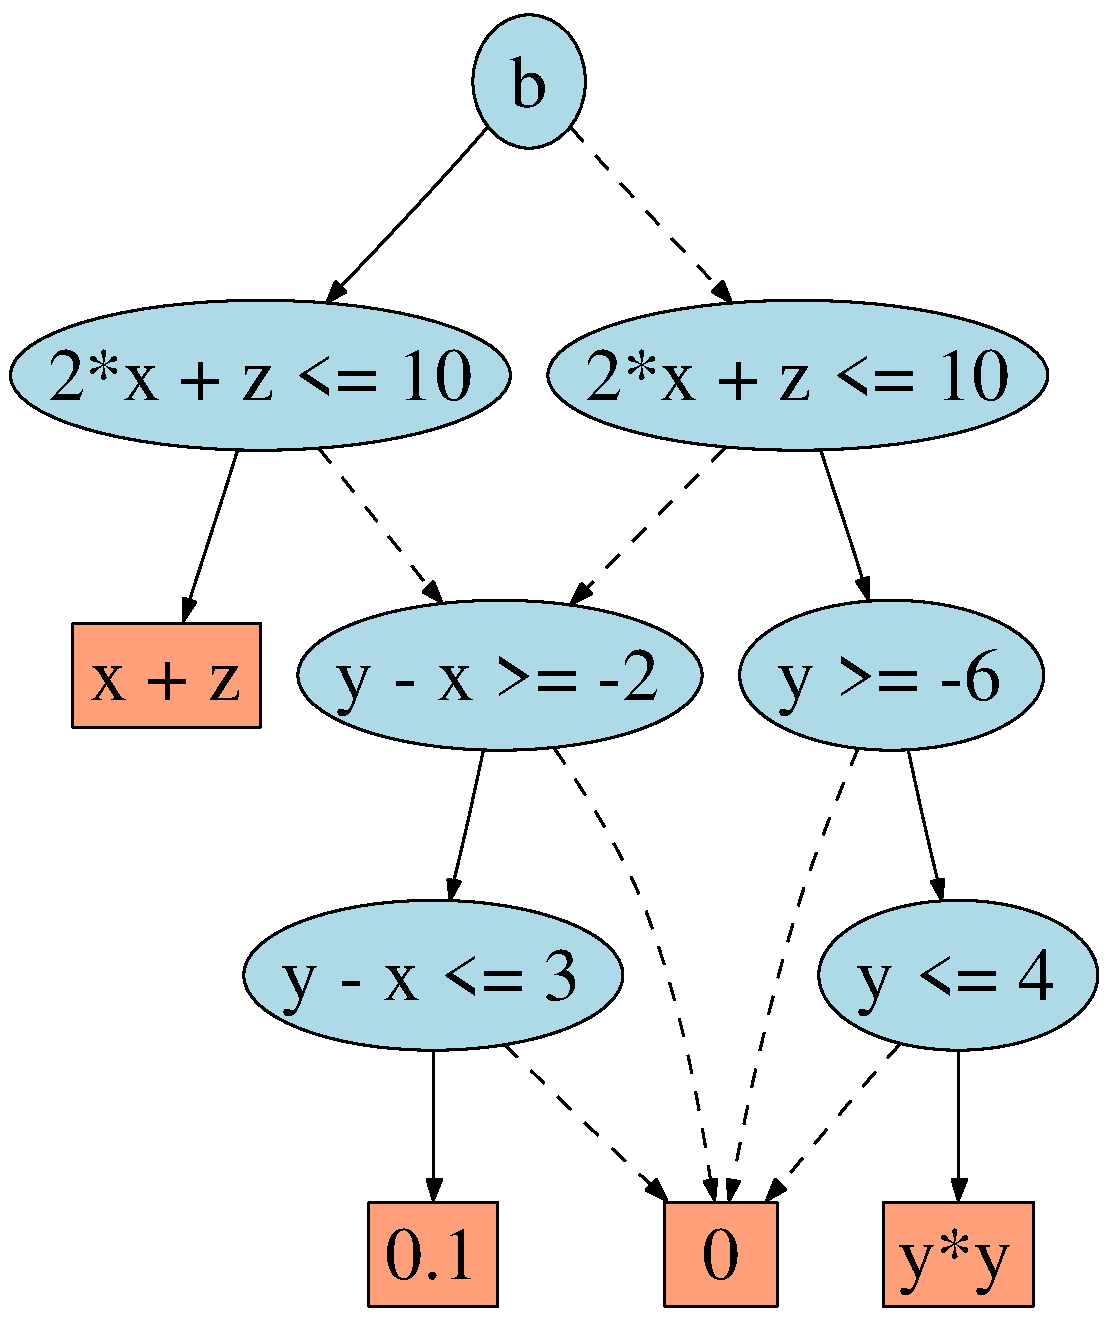
\includegraphics[width=.25\textwidth]{Figs/norm_unif.pdf}
\end{center}
\vspace{-2mm}
\caption{\footnotesize An XADD example.% in Figure~\ref{fig:xadd_tree}.
} \label{fig:xadd}
\vspace{-4mm}
\end{figure}
%%%%%%%%%%%%%%%%%%%%%%%%%%%%%%%%%%%%%%%%%%%%%%%%%%%%%%%%%%%%%%%%%%%%%%%%%%

The XADD is like an algebraic decision 
diagram (ADD)~\cite{bahar93add} except that (a) the decision
nodes can have arbitrary inequalities (one
per node) and (b) the leaf nodes can represent arbitrary functions.
The decision nodes still have a fixed order from root to leaf
and the standard ADD
operations to build a canonical ADD (\textsc{Reduce}) and 
to perform a binary operation on two ADDs (\textsc{Apply}) 
still apply with minor modifications in the case of XADDs. 

Of particular importance is that the XADD is a directed acyclic graph
(DAG), and hence is often much more compact than a tree
representation, e.g., as demonstrated in Figure~\ref{fig:xadd}.
Furthermore, one can use the feasibility checker of an LP solver to
incrementally prune unreachable branches in the XADD DAG --- an
operation crucial for maintaining XADD
compactness and minimality~\cite{uai11}.  We remark that not only are
XADDs compact on account of their reconvergent DAG structure (each
path from root to leaf would be a separate case partition), but that
all unary and binary operations on XADDs can directly exploit this
compact DAG structure for efficiency.

All XADD operations except for definite integration have been defined
previously; we note that unlike ADDs, some XADD operations like
$\max(\cdot,\cdot)$ and $\min(\cdot,\cdot)$ can introduce out-of-order
decisions which can be easily detected and repaired as discussed
in~\cite{uai11}.  Extending the definite integration operation to
XADDs is straightforward: treating each XADD path from root to leaf
node as a single case partition with conjunctive constraints,
$\int_{v=-\infty}^{\infty}$ is performed at each leaf  
and the result accumulated via the
$\oplus$ operation to compute~\eqref{eq:int_decomp}.

\subsection{Computational Complexity}

For a graphical model inference algorithm like SVE, it is a natural
question to wonder if space and computation time can be bounded in
terms of the tree-width of the underlying graph, as for purely
discrete models.  The short answer is no.  While a factor over many
variables may be represented compactly as a piecewise expression
(unlike, e.g., a tabular enumeration in the discrete case), one can
generally only upper bound the number of pieces needed in a case
expression (and hence computation time and space) as an exponential
function of the number of primitive binary operations
($\oplus,\otimes,\max,\min$) used by SVE --- assuming the PPFG has
some factor with at least two non-zero case partitions.  Since
one definite integral during SVE can easily require 10's or 100's of
primitive case operations, one can see that either SVE will be intractable
\emph{or} that these worst-case upper bounds are extremely loose when
using data structures like the XADD.  Fortunately, the latter proves
to be the case as shown next in the empirical results.

%\vspace{-3mm}

\section{Empirical Results}

%\vspace{-1mm}

%%%%%%%%%%%%%%%%%%%%%%%%%%%%%%%%%%%%%%%%%%%%%%%%%%%%%%%%%%%%%%%%%%%%%%%%%%
\begin{figure*}[t!]
\begin{center}
\vspace{-1mm}
%{\tiny
\begin{tabular}{ccc}
\vspace{-3mm}
\hspace{-8mm} 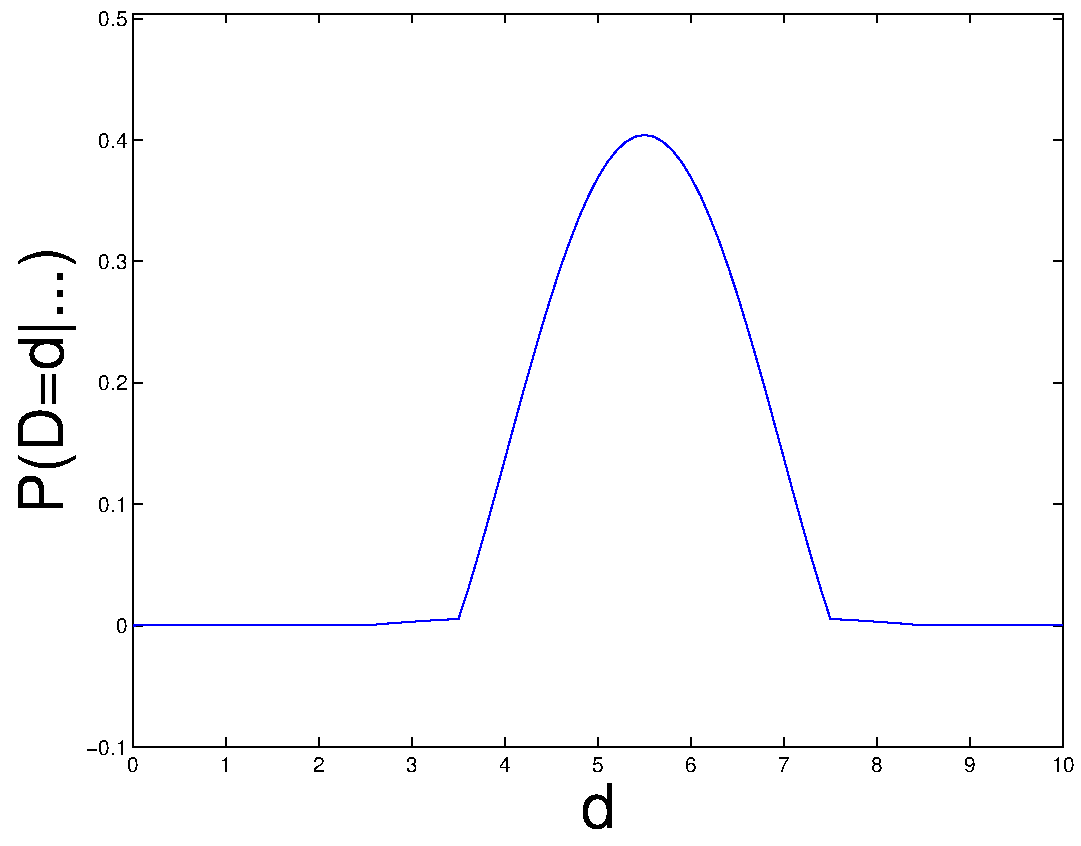
\includegraphics[width=90pt]{Figs/r1.pdf} & \hspace{-6mm} 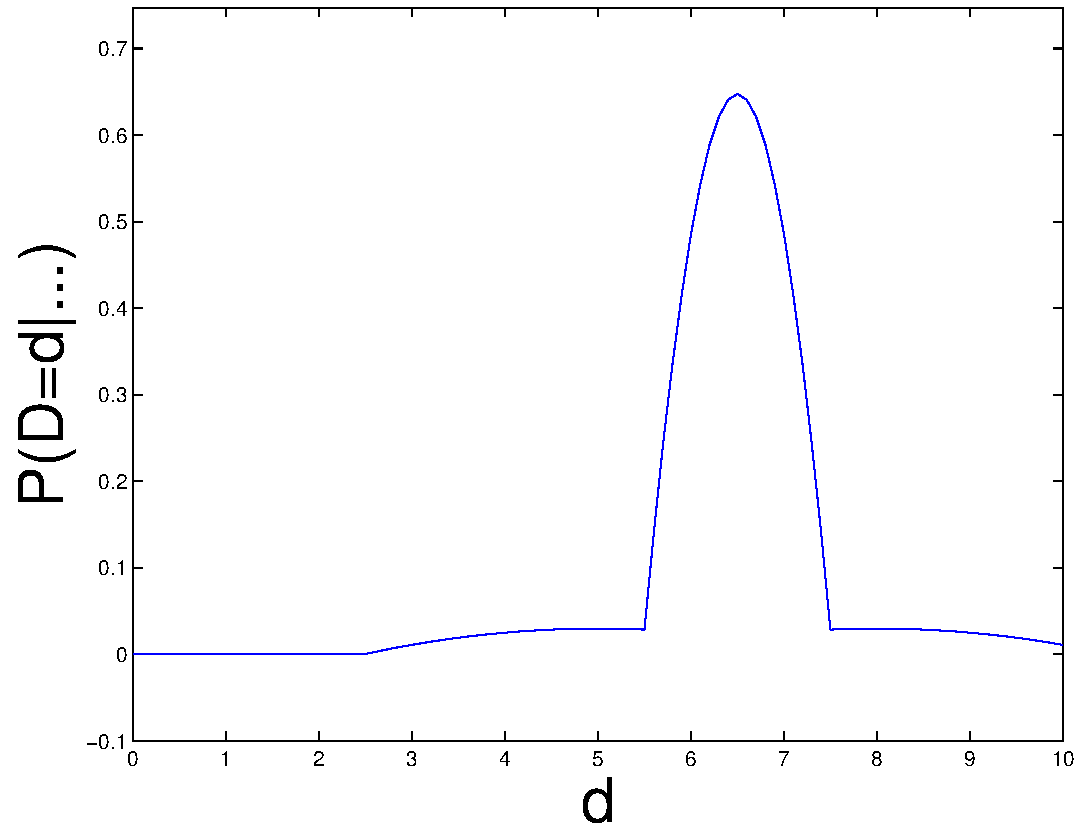
\includegraphics[width=90pt]{Figs/r2.pdf} & \hspace{-10mm} 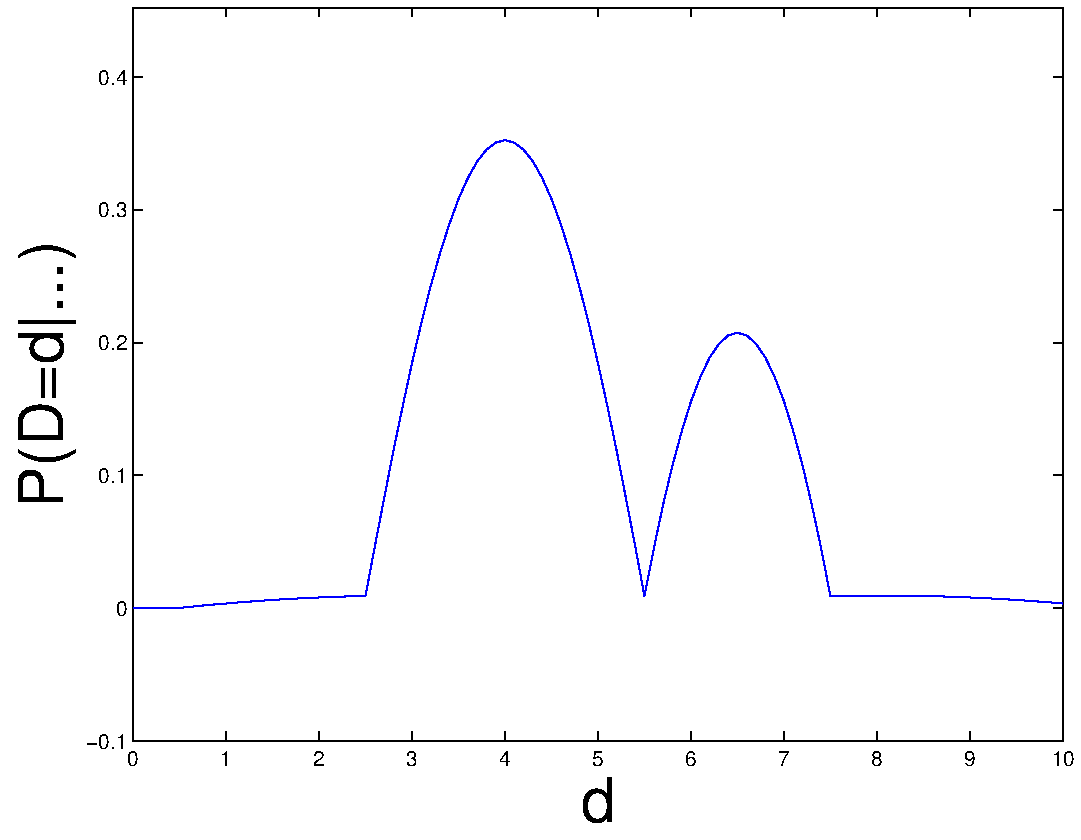
\includegraphics[width=90pt]{Figs/r3.pdf} \\  
\vspace{4mm}
{\small$\E[D|x_1=6, x_2=5] = 4.98$} & {\footnotesize$\E[D|x_1=8, x_2=5]= 6.0$} & \hspace{-3mm} {\footnotesize$\E[D|x_1=5, x_2=3, x_3=8] = 4.39$}\\
\vspace{-2mm}
\hspace{-8mm} 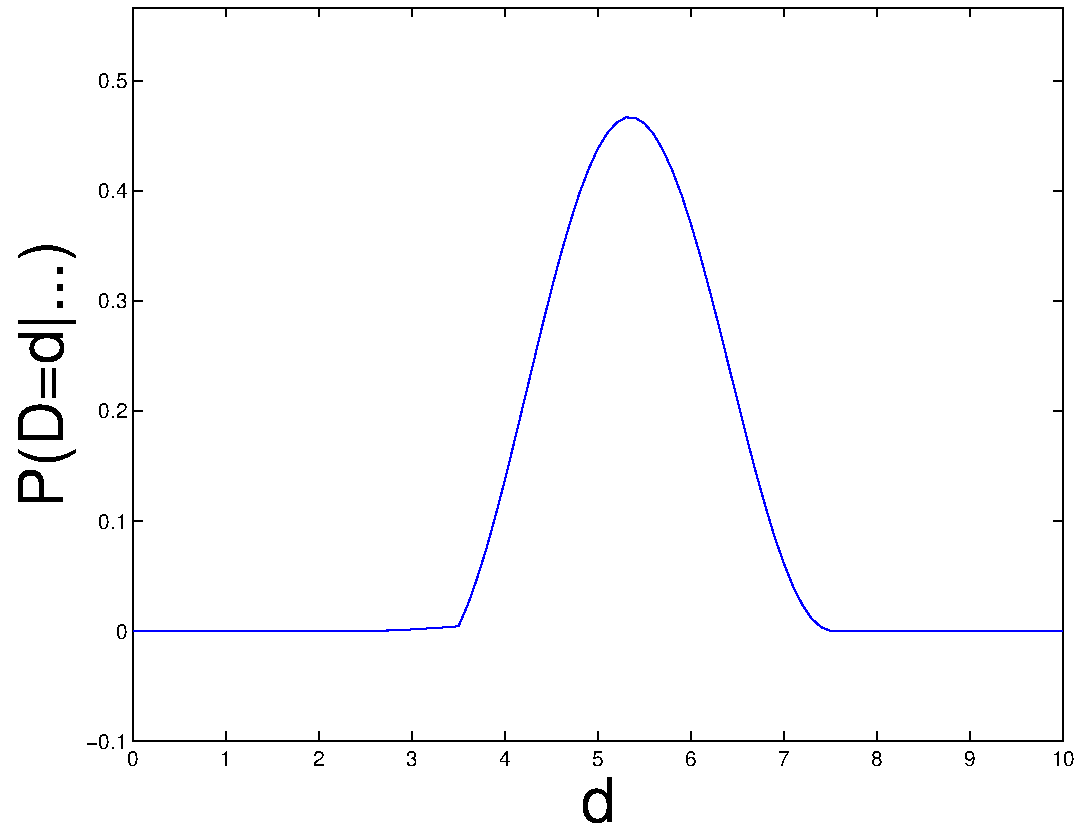
\includegraphics[width=90pt]{Figs/r4.pdf} & \hspace{-6mm} 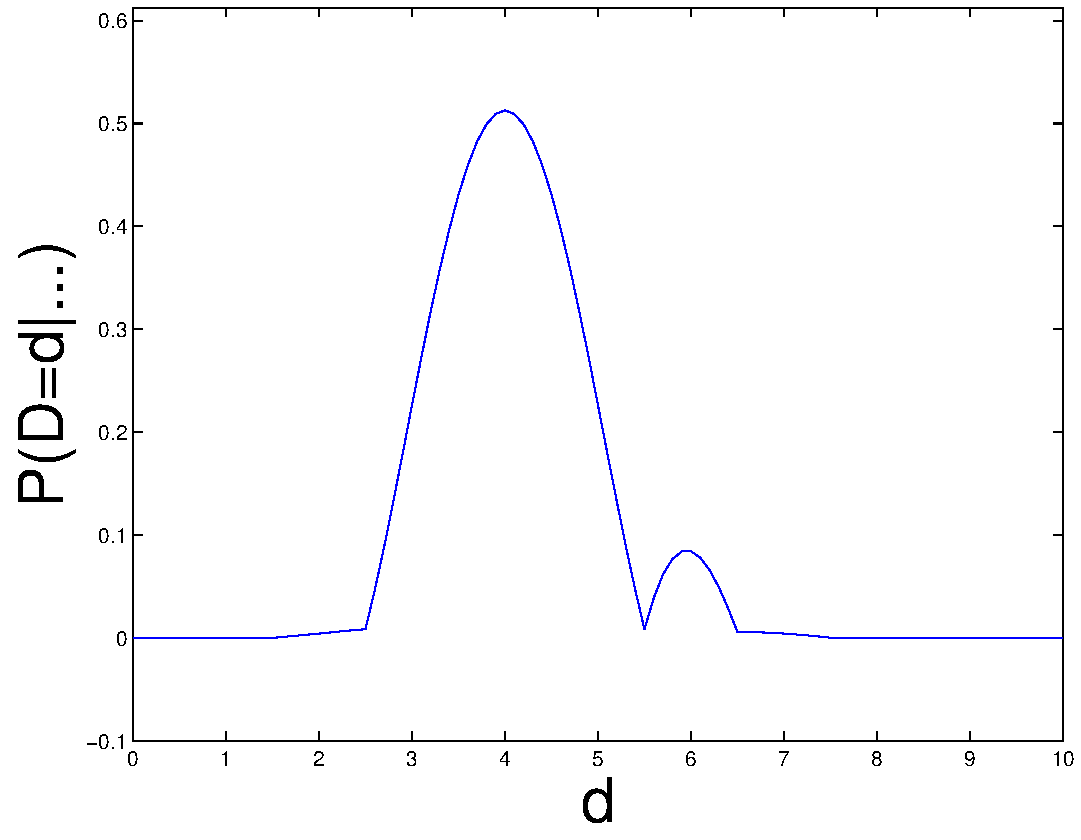
\includegraphics[width=90pt]{Figs/r5.pdf} & \hspace{-10mm} 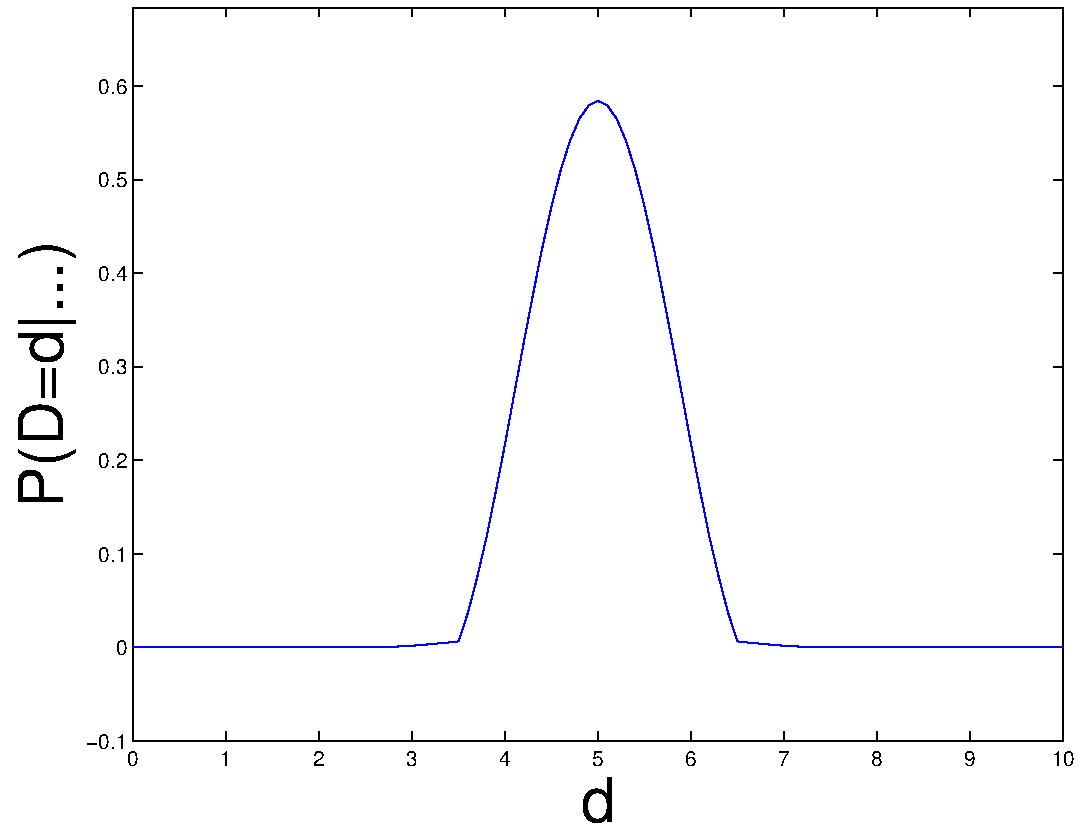
\includegraphics[width=90pt]{Figs/r6.pdf} \\
\vspace{4mm}
{\footnotesize$\E[D|x_1=5, x_2=5, x_3=6] = 4.98$} & {\footnotesize$\E[D|x_2=1, x_2=3, x_3=4, x_4=8] = 5.45$} & {\footnotesize$\E[D|x_1=5, x_2=4, x_3=6, x_4=5] = 4.89$} 
\end{tabular}
\end{center}
\vspace{-4mm}
\caption{\footnotesize Queries for {robot localization}.  The diagrams show $p(d|\vec{e})$ vs. $d$ for the given evidence $\vec{e}$ shown below each diagram along with the exactly computed expectation $\E[D|\vec{e}]$ for this distribution.} \label{fig:dist}
\end{figure*}
%%%%%%%%%%%%%%%%%%%%%%%%%%%%%%%%%%%%%%%%%%%%%%%%%%%%%%%%%%%%%%%%%%%%%%%%%%

In this section we present proof-of-concept experiments for the {robot
localization} graphical model provided in the introduction and
a basic discrete/continuous {tracking} task in
Figure~\ref{fig:gm3}.  Our objectives in this section are to show that
the previously defined {exact} inference methods can work with
reasonably sized graphical models having multiple continuous and
discrete variables with complex piecewise polynomial distributions
and that SVE can exactly compute the highly complex, multi-modal
queries in an {exact} functional form --- a milestone in 
exact closed-form inference for graphical models
with such complex combinations of distributions.

{\bf Localization:} 
For the {robot localization} task, we plot the posterior over the
distance $d \in D$ given various observations in
Figure~\ref{fig:dist}.  What is noteworthy here is the interesting
multi-modal nature of these plots. Recalling the discussion in the
introduction, the range finder was modeled with various error modes;
because of these models, the posterior plots demonstrate the different
combinatorial possibilities that each measurement was accurate or
noise with the various peaks in the distribution weighted according to
these probabilities.  Despite the multi-modal nature of these
distributions, the conditional expectation of $D$ can be computed
exactly and is shown below each posterior.  

We note that in a Bayesian
risk setting, where these posterior beliefs may be multiplied by some
position-based risk function (e.g., one that increases with proximity
to stairwells), it is important to have this true multi-modal
posterior rather than an inaccurate unimodal approximation.  And while
sampling may work well for fixed expected risk calculations, if the
evidence is changing or one wants to perform sensitivity analysis of
risk subject to differing evidence (i.e., conditioning on unassigned
evidence), one must collect samples for each specific evidence case
under consideration.

{\bf Tracking:} The {tracking} graphical model and (conditional)
distributions are shown in Figure~\ref{fig:gm3} and works as follows:
an object has hidden state $x_i \in \R$ defining it's $x$ position
that is sampled for time steps $i = 1 \ldots t$.  On every time step a
noisy observation $o_i \in \R$ is received regarding the position of
the object.  Also at every time step, a variable $b_i$ indicates
whether the sensor is broken ($1$) or not ($0$).  A sensor fails with
probability 0.2 and stays broken once it breaks.  If the sensor is not
broken, the observation model for $o_i$ is a symmetrical triangular
distribution centered on the underlying state $x_i$; if it is broken the
observation model is an asymmetric triangular distribution with a peak
at the true $x_i$ state, but biased to underestimate.  The initial position 
$x_1$ is uniformly distributed between $0$ and $10$ 
and each subsequent $x_{i+1}$ is sampled
from a truncated Gaussian centered on $x_i$.

%%%%%%%%%%%%%%%%%%%%%%%%%%%%%%%%%%%%%%%%%%%%%%%%%%%%%%%%%%%%%%%%%%%%%%%%%%
\begin{figure*}[t!]
\begin{center}
%\vspace{-1mm}
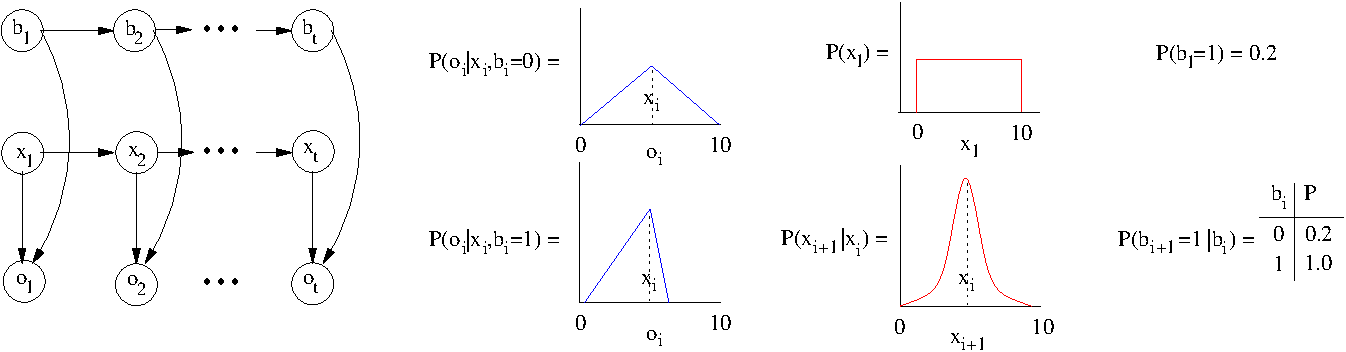
\includegraphics[width=.95\textwidth]{Figs/gm3.pdf}
\end{center}
\vspace{-4mm}
\caption{\footnotesize The {tracking} graphical model and all conditional probabilities.} \label{fig:gm3}
%\vspace{-2mm}
\end{figure*}
%%%%%%%%%%%%%%%%%%%%%%%%%%%%%%%%%%%%%%%%%%%%%%%%%%%%%%%%%%%%%%%%%%%%%%%%%%

%%%%%%%%%%%%%%%%%%%%%%%%%%%%%%%%%%%%%%%%%%%%%%%%%%%%%%%%%%%%%%%%%%%%%%%%%%
\begin{figure*}[t!]
%\vspace{-3mm}
\begin{center}
\begin{tabular}{ccc}
\hspace{-3mm} 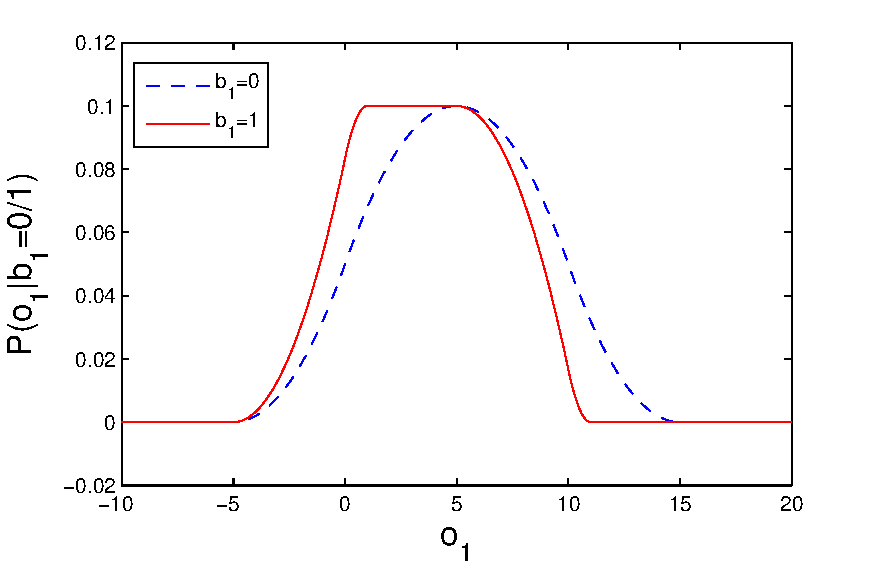
\includegraphics[width=170pt]{Figs/radar_o1_fix.pdf} & \hspace{-5mm} 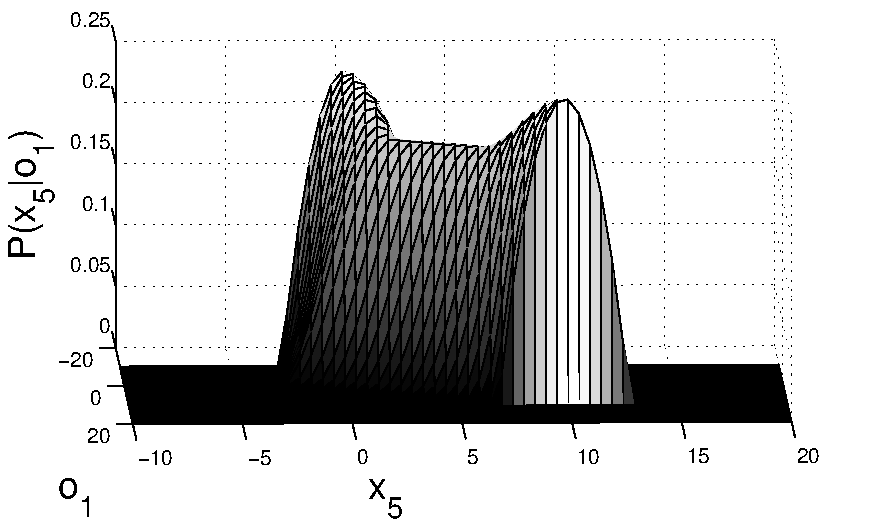
\includegraphics[width=170pt]{Figs/radar_x5_o1_3d.pdf} & \hspace{-4mm} 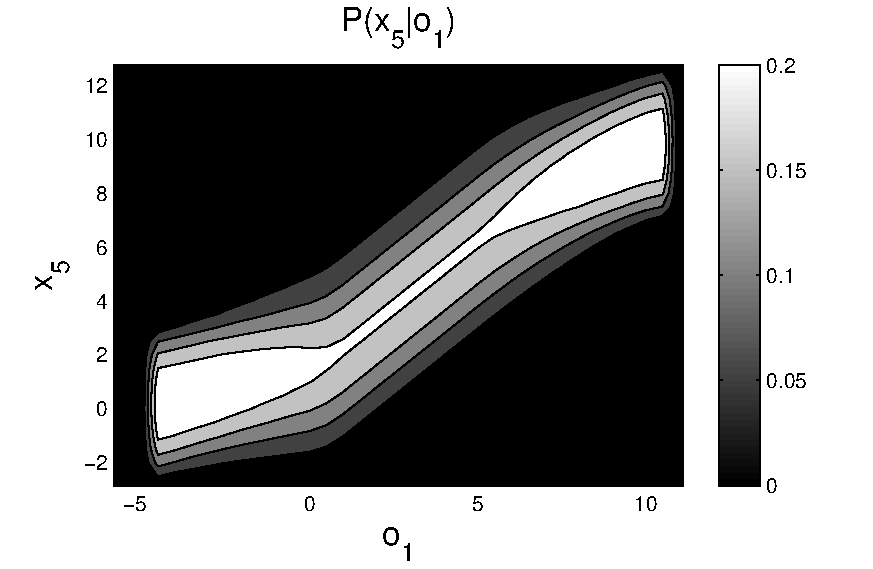
\includegraphics[width=170pt]{Figs/radar_x5_o1.pdf}\\ 
(a) & (b) & (c) \\
\multicolumn{3}{c}{}
\end{tabular}
\end{center}
\vspace{-6mm}
\caption{\footnotesize Plots of query and evidence variables for three
queries in \emph{tracking}: (a)  $p(o_1|b_1=0)$ (blue dash)
and $p(o_1|b_1=1)$ (red solid).
(b) $p(x_5|o_1)$ as a 3D plot, and (c) $p(x_5|o_1)$ as a contour plot.}
\label{fig:track}
%\vspace{-4mm}
\end{figure*}
%%%%%%%%%%%%%%%%%%%%%%%%%%%%%%%%%%%%%%%%%%%%%%%%%%%%%%%%%%%%%%%%%%%%%%%%%%

In Figure~\ref{fig:track}, we show results for three queries in the
{tracking} model.  Result (a) demonstrates an asymmetric posterior 
while results (b) and (c) demonstrate the
complex multi-modal posterior distribution over $x_3$ conditioned
on uninstantiated continuous evidence $o_1$ and the ability of the
SVE inference algorithm to compute this in an exact closed-form.  All
of these queries completed in under 1 minute demonstrating that
despite the complex symbolic manipulations involved and 
multidimensional/multimodal inference results, the SVE method
can effectively compute closed-form exact inference for this non-Gaussian
tracking task.

The important point to observe here in both Figures~\ref{fig:dist} and
\ref{fig:track} is that using SVE we are able to derive various
multi-modal and highly irregular posterior distributions in an exact
functional form.  And due to our symbolic form, we are able to derive
this distribution as a function of uninstantiated evidence as in 
Figures~\ref{fig:track}(b,c) --- inference that is not easily
done (if at all) via standard sampling or numerical integration
techniques.  Such symbolic forms are useful when we want to analyze
arbitrary variable dependencies in complex systems with sophisticated
distributions that can be specified (or arbitrarily approximated) as
PPFGs.

%One interesting thing to observe here in these experiments is the clear advantage of using 

%\vspace{-5mm}

\section{Related Work}

%\vspace{-5mm}

Almost all prior work on continuous variable graphical models --- with
the exception of Kalman filtering~\cite{kalman_filter} and other jointly 
Gaussian models~\cite{Weiss99correctnesof} --- has focused on
\emph{approximate} or \emph{non-closed-form, exact} inference.
Such methods for non-Gaussian continuous graphical model inference include 
\begin{itemize}
\item \emph{Discretization}: arbitrary accuracy but subject to the curse
of dimensionality,
\item \emph{Numerical Integration}: arbitrary accuracy but 
subject to the curse
of dimensionality, also only applies to instantiated
continuous evidence --- rather
than uninstantiated evidence as shown for
the SVE query in Figures~\ref{fig:track}(b,c), 
\item \emph{(MCMC) Sampling}: exemplified in the expressive
BUGS language and inference~\cite{bugs}, aymptotically unbiased 
but only applies to instantiated evidence and 
known to be slow to converge when probabilities
are nearly deterministic (note that SVE is unaffected by this), 
\item \emph{Projected Message Passing} 
such as variational inference~\cite{variational} and expectation
propagation~\cite{minka_ep} that can produce a functional form for a
query result, but with an \emph{a priori} assumed projective distribution
(often Gaussian) that may not be appropriate in practice,
cf. Figures~\ref{fig:track}(b,c), and 
\item \emph{Mixtures of Truncated Exponentials (MTEs)}: 
an approach introduced in~\cite{moral_mtes} not unlike that taken here
and further developed extensively in the approximate case -- even with 
trees~\cite{moral_tree_mtes,penniless_tree_mte,cobb_approx_mtes},
but only for non-oblique pieces (hyper-rectangular 
piece boundaries) that may require arbitrary space
to accurately approximate functions that can be exactly
represented with oblique pieces as 
in Figures~\ref{fig:track}(b,c).
\end{itemize}
In short, it seems that little progress has been made in
\emph{closed-form exact} inference of results in a functional form for
\emph{expressive} non-Gaussian joint distributions and uninstantiated
continuous evidence --- as done for the oblique piecewise polynomial
distributions in this paper.

\section{Concluding Remarks}

SVE and its PPFG formalism using oblique piecewise polynomials 
represents a novel and expressive class of \emph{non-Gaussian} factors
for which integration is closed-form, thus enabling exact symbolic 
inference for any probability queries and expectations in this
model.  Most realistic distributions have bounded support and can be
arbitrarily approximated by piecewise polynomials, hence this work
opens up the possibility of exact solutions (or arbitrary
approximations thereof) in discrete/continuous graphical models for
which previous exact solutions were not available.  As
such, we believe that SVE provides a significant step forward and a
new alternative for the difficult task of \emph{exact closed-form} inference
in discrete and continuous graphical models.

%We crucially note that SVE is \emph{not} limited to piecewise
%polynomial models, but that once more general expressions are
%introduced, we cannot guarantee that symbolic integrations will always
%be possible.  Nonetheless, when all of the integrations in more
%general models can be computed symbolically (and much progress has
%been made in recent decades on automated symbolic integration), the
%SVE result will be \emph{exact and closed-form}.  Furthermore, if a certain
%function class is truly non-integrable, it may still be
%well-approximated by other integral function classes; this paves the way
%for the application of SVE to an extremely 
%expressive range of discrete/continuous graphical models.  Hence, we
%believe this paper is only the tip of the iceberg for SVE and its
%future applications.

{\small
\section*{Acknowledgements}

NICTA is funded by the Australian Government as represented by
the Department of Broadband, Communications and the Digital
Economy and the Australian Research Council through the ICT
Centre of Excellence program.}

\bibliography{sve}
\bibliographystyle{aaai}

\end{document}
